% Warum manuell
Viele Studien in der Literatur haben Klassifizierungsmethoden verwendet, um die Datensicherheit in der Cloud zu gewährleisten. Die vorgeschlagenen Lösungen lassen sich in zwei Klassen einteilen: die manuelle Klassifizierung, die vom Nutzer festgelegt wird, und die automatische Klassifizierung, bei der ein Algorithmus zum Einsatz kommt.

Die manuelle Datenklassifizierung ist trotz Fortschritte bei automatisierten Technologien eine gängige Methode. In einigen Fällen, wie bei der Klassifizierung von Informationen wie geistigem Eigentum oder Geschäftsgeheimnissen, bleibt die manuelle Klassifizierung erforderlich. Menschen sind in der Lage, leicht die Kategorien, Kontexte, Strukturen und Zustände der Daten ganzheitlich zu berücksichtigen. Außerdem kann die manuelle Klassifizierung für kleinere Unternehmen kostengünstig sein \cite{Divadari.2023}\cite{Alsuwaie.2021}.

% warum schwierig (aufwändig, fehlerbehaftet, Big Data)
Die manuelle Klassifizierung von Daten ist jedoch sehr anfällig für menschliche Fehler und Inkonsistenzen. Die Subjektivität der Menschen kann zu inkonsistenten Klassifizierungen führen, was die Genauigkeit und Zuverlässigkeit der Sicherheitsmaßnahmen beeinträchtigen kann. Zudem kann eine unzureichende Genauigkeit zu unvollständigen oder falschen Klassifizierungen führen. Im Normalfall werden Daten bei ihrer Erstellung klassifiziert, doch sie können sich im Laufe der Zeit ändern, wodurch die ursprüngliche Klassifizierung veraltet und nicht mehr richtig sein kann. Die manuelle Einordnung von großen Datenmengen kann sehr zeitaufwändig und arbeitsintensiv sein und ab einer bestimmten Größe nicht mehr manuell verarbeitet werden. Manuelle Prozesse können die Anpassungsfähigkeit und schnelle Reaktion auf sich ändernde Geschäftsanforderungen reduzieren \cite{Venhorst.2019}.

Aufgrund der wachsenden Datenmengen und der zunehmenden Komplexität der Informationssicherheitsanforderungen erscheint die automatisierte Datenklassifizierung häufig als effizientere Lösung, die eine genauere und konsistentere Identifizierung sensibler Daten ermöglicht.

\subsection{Methoden der automatischen Datenklassifizierung}
% warum automatisiert
Der Prozess, bei dem maschinelle Algorithmen und Technologien verwendet werden, um Daten automatisch zu identifizieren, zu kategorisieren und entsprechend ihres Sensitivität zu klassifizieren, wird als automatische Datenklassifizierung bezeichnet. Diese Methode verwendet maschinelles Lernen, Mustererkennung oder künstliche Intelligenz, um Daten zu analysieren und automatisch geeignete Klassifizierungen zuzuweisen.
Die aktuellen Techniken in der Data Leakage Prevention können allgemein in zwei Kategorien eingeteilt werden: inhaltsbasierte Analyse und kontextbasierte Analyse. Methoden, die auf dem Inhalt basieren, untersuchen den Inhalt von Daten anhand von Merkmalen sensibler Informationen wie regulären Ausdrücken und Datenfingerabdrücken. Inhaltsbasierte Methoden verwenden vorhersehbare Muster wie z.B. IP-Adressen oder E-Mail-Adressen, um sensible Daten zu erkennen. Kontextbasierte Techniken identifizieren vertrauliche Daten anhand von Merkmalen im Zusammenhanf mit den überwachten Daten. Der kontextbasierte Ansatz ist damit effektiver für vertrauliche Daten ohne vorhersehbare Muster \cite{Guo.2021}\cite{Gugelmann.2015}\cite{Kuzina.2023}. Um sensible Informationen umfassender und genauer zu extrahieren, sollten daher verschiedene Methoden angewendet werden. Die Tabelle \ref{t:methoden} zeigt die am häufigsten verwendeten Methoden in der Literatur. In Kapitel \ref{k:content} und \ref{k:context} werden die inhaltsbasierten und kontextbasierten Methoden genauer erläutert.

%Tabelle mit content-based vs. context-based
\begin{table}[htbp]
    \normalsize
    \caption{Methoden der automatischen Datenklassifizierung. Quelle: eigene Darstellung.}
    \label{t:methoden}
    \begin{center}
        \begin{tabulary}{15cm}{|L|L|}
            \hline
            \textbf{Kategorie}                           & \textbf{Methode} \bigstrut  \\
            \hline
            \hline
            \multirow{9}{4em}{basierend auf dem Inhalt}  & rule-based \bigstrut[t]     \\
            & ML Classifier               \\
            & Vector based                \\
            & Frequency method            \\
            & Fingerprint                 \\
            & Neuronal Network            \\
            & Statistic Analysis          \\
            & Text Clustering             \\
            & ML K-NN                     \\
            \hline
            \multirow{5}{4em}{basierend auf dem Kontext} & Deep Learning  \bigstrut[t] \\
            & Graph-based                 \\
            & ML semantic analysis        \\
            & BiLSTM                      \\
            & Cassed                      \\
            \hline
        \end{tabulary}
    \end{center}
\end{table}

\subsubsection{content-based} \label{k:content}

\paragraph{regelbasierte Methoden}
% rule-based/regular-matching/Dictionary
Eine einfache und häufig angewendete Technik zur automatischen Datenklassifizierung basiert auf einem Wörterbuch oder einer Regel, die im Wesentlichen den gegebenen Text mit einer Liste vordefinierter regulärer Ausdrücke und Schlüsselwörter abgleicht. Diese Methode verwendet vordefinierte Regeln und Bedingungen, um bestimmte Datentypen oder Muster automatisch zu identifizieren und zu klassifizieren. Diese Regeln können auf verschiedenen Merkmalen wie Schlüsselwörtern, Mustern, Dateiformaten oder spezifischen Attributen wie Datumsangaben basieren \cite{Ong.2017}.
Die Identifikation von Kreditkartennummern in Textdokumenten ist ein Beispiel für die Verwendung regelbasierter Methoden. Zur Erkennung kann ein regulärer Ausdruck verwendet werden, der die Zeichenfolge nach dem Muster einer Kreditkartennummer definiert. Muster in regulären Ausdrücken umfassen meistens normale Zeichen mit wörtlicher Bedeutung und Metazeichen, um ein Erkennungsmuster zu bilden \cite{Alneyadi.2016}.
Regeln können sich auch auf bestimmte Schlüsselwörter oder Phrasen beziehen, die auf personenbezogene Informationen wie \glqq Sozialversicherungsnummer\grqq \:oder \glqq vertraulich\grqq \:hinweisen können.
Der Vorteil regelbasierter Methoden liegt in ihrer klaren Struktur und der Möglichkeit, spezifische Anforderungen und Richtlinien der Organisation abzubilden. Sie ermöglichen eine präzise und konsistente Klassifizierung von Daten gemäß vordefinierten Sicherheitsstandards. Da die Klassifizierung auf klaren, vorher festgelegten Regeln basiert, ermöglichen regelbasierte Ansätze auch eine gewisse Transparenz und Nachvollziehbarkeit.
Jedoch können regelbasierte Methoden bei der Verarbeitung komplexer und sich verändernder Datenmuster weniger nützlich sein, da die Regeln schnell unpraktisch werden, wenn Datenformate, Kontext, Wortvariationen und Abkürzungen kombiniert werden müssen. Der Einsatz dieser Methode erfordert auch ein gut definiertes und gepflegtes Wörterbuch und Regelsatz. AAußerdem wird der semantische Kontext der Wörter bei einem reinen Textabgleich nicht berücksichtigt, was zu einer geringen Genauigkeit der Klassifizierung führen kann \cite{Ong.2017}.
Trotzdem bieten regelbasierte Ansätze eine grundlegende und robuste Methode zur Sicherstellung einer konsistenten Datenklassifizierung.

\paragraph{Data Fingerprinting}
Data Fingerprinting oder auch Document Fingerprinting erstellt eindeutige Fingerabdrücke für bestimmte Datenfragmente oder ganze Dateien. Diese Fingerabdrücke sind eindeutige Identifikatoren für die entsprechenden Daten und werden genutzt, um sensible Daten zu identifizieren und automatisch zu klassifizieren. Eindeutige Fingerabdrücke für Wörter, Sätze oder ganze Dateien werden mithilfe von Wortmustern aus regulären Ausdrücken oder vordefinierten Wörterbüchern erstellt und als Vorlage für sensible Daten verwendet. Diese Fingerabdrücke können dann verwendet werden, um Fingerabdrücke von nicht-klassifizierten Daten zu vergleichen und zu klassifizieren.
Häufig werden Hash-Funktionen wie MD5 oder SHA1 verwendet, um Datenfingerprints zu erstellen, die eine algorithmisch generierte Zeichenfolge fester Größe für die Daten darstellen. Die Hashes von zwei Dateien unterscheiden sich jedoch, sobald nur ein Zeichen verändert wurde \cite{Alneyadi.2016}. Ein weiterer Ansatz ist deshalb das \glqq Fuzzy-Hashing\grqq. Hierbei werden die Daten in Blöcken verarbeitet, wodurch die Hash-Ausgabe bei ähnlichen Daten größtenteils übereinstimmende Blöcke enthält. So kann die prozentuale Ähnlichkeit mithilfe einer mathematischen Vergleichsfunktion bestimmt werden \cite{Shu.2015}.

Sowohl im Speicher als auch bei Netzwerkübertragungen oder bei Verwendung kann das Data Fingerprinting sensible Daten erkennen. Der Fingerabdruck ist in manchen Fällen jedoch keine zuverlässige Methode. Die Klassifizierung funktioniert nicht, wenn die Daten verschlüsselt oder passwortgeschützt sind oder der Inhalt nicht eindeutig mit dem Fingerabdruck übereinstimmt. Außerdem ist es notwendig, dass die Vorlagen kontinuierlich aktualisiert werden und der Ansatz kann bei großen Datenmengen ressourcenintensiv sein.

\paragraph{Clusteranalyse}
% auf Basis von wenigen manuell klassifizierten Daten können Cluster gebildet werden
Die Clusteranalyse ist eine Datenanalysetechnik aus dem Bereich maschinellen Lernens. Clustering gehört zur Gruppe der Unsupervised Learning Methoden, bei der die Methode ohne vorher definierte Zielwerte Muster in Eingabedaten erkennt. Beim Clustering werden unsortierte Informationen ohne vorheriges Datentraining nach Ähnlichkeiten, Mustern und Unterschieden gruppiert. Im Bezug auf die Klassifikation von sensiblen Daten wird die Clusteranalyse auf die vorhandenen Daten in einem Unternehmen angewandt. Die entstandenen Cluster enthalten dann jeweils ähnliche Dokumente gemäß einer Ähnlichkeitsmetrik wie der euklidischen Distanz oder der Cosinus-Ähnlichkeit \cite{Suyal.2014}.
Zur Verwendung der Clusteranalyse als Klassifikator müssen vor der Analyse relevante Merkmale oder Attribute definiert werden, anhand derer sensible Daten erkannt werden können. Anschließend können die Daten in einem Cluster, das bestimmte Merkmale enthält, jeweils klassifiziert werden.

Zwei übliche Clustering-Methoden ist das hierarchische Clustering und das distanzbasierte Clustering. Das hierarchische Clustering wird meist für Text-Clustering verwendet, indem jedes Dokument basierend auf seiner Ähnlichkeit sukzessive in einem vordefinierten Cluster zusammengeführt wird. Dabei entsteht eine Clusterhierarchie, die über ein Dendrogramm als Baumstruktur dargestellt werden kann. Abbildung \ref{f:clustering_daten} zeigt ein Beispiel-Datensatz aus den Objekten a bis f. Dabei liegen die Objekte b und c sowie d und e sehr dicht zusammen. Der Clustering-Algorithmus fasst nun nach und nach zuerst die Objekte mit der kürzesten Distanz, dann die nächsten Objekte oder Cluster zusammen, bis zur Gesamtmenge. So wird ein Baum wie in Abbildung \ref{f:clustering_baum} erstellt, dessen Blätter Cluster repräsentieren, die nur ein einzelnes Objekt der Datenmenge beinhalten und dessen Wurzel ein einziges Cluster mit allen Objekten darstellt. Die Kanten zwischen den Knoten enthält zudem ein Attribut, das die Distanz zwischen den beiden Clustern definiert. Je nachdem, wie groß oder klein die Anzahl der Cluster gewählt werden sollen, können die Cluster auf einer Knoten-Ebene verwendet werden \cite{Suyal.2014}.

\begin{figure}[htbp]
    \centering
    \begin{subfigure}[b]{0.47\linewidth}
        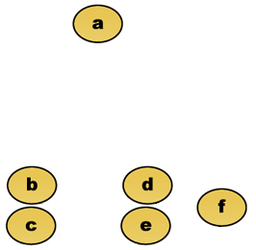
\includegraphics[width=\linewidth]{\figdir/clustering_daten}
        \caption{Datensatz. Quelle: In Anlehnung an \cite{Bonthu.2023}.}
        \label{f:clustering_daten}
    \end{subfigure}
    \hfill
    \begin{subfigure}[b]{0.47\linewidth}
        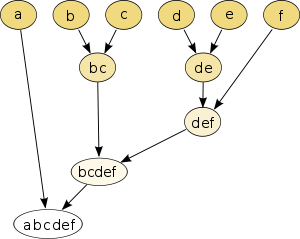
\includegraphics[width=\linewidth]{\figdir/clustering_dendrogramm}
        \caption{Dendrogramm. Quelle: In Anlehnung an \cite{Bonthu.2023}.}
        \label{f:clustering_baum}
    \end{subfigure}
\end{figure}

Aufgrund seiner Einfachheit und Flexibilität wird hierarchisches Clustering häufig verwendet und bietet den Vorteil, jede Art von Ähnlichkeitsmessungen durchzuführen. Der größte Nachteil dieses Algorithmus besteht darin, dass es schwierig ist, zu bestimmen, welche Baum-Knoten-Ebene das optimale Clustering darstellt.

% TODO: distanzbasierte Clustering k-mean

\paragraph{Maschinelles Lernen}
% ML classifier

\paragraph{Deep Learning}
% neuronal network


\subsubsection{context-based} \label{k:context}
% deep learning
% TF-IDF https://www.analyticsvidhya.com/blog/2021/09/creating-a-movie-reviews-classifier-using-tf-idf-in-python/
% graph based -> CBDLPA
% ML semantic analysis
% BERT-BiLSTM-Attention Model (Guo)
% BERT: Cassed

\paragraph{statistische Analyse}
% N-Gramm-Analyse
% Termgewichtungsanalyse

\subsubsection{Kombinationen} \label{k:kombi}
% Quasi Identifier -> Kombi aus manueller Klassifizierung und Content/Kontext


\subsection{Anwendung in der Cloud Security}
% wofür ist das dann gut

\subsubsection{Labeling für andere Maßnahmen}
% verschlüsselung
% Access Rights
% Versenden
% fingerprint


\subsubsection{Anwendungsbeispiele}
% BrowserFlow
% DocGuard?